\documentclass[11pt]{article}
\usepackage{../../local}
\usepackage{chemformula}


\newcommand{\classcode}{Physics 112}
\newcommand{\classname}{Introduction to Statistical Mechanics}
\renewcommand{\maketitle}{%
\hrule height4pt
\large{Eric Du \hfill \classcode}
\newline
\large{HW 01} \Large{\hfill \classname \hfill} \large{\today}
\hrule height4pt \vskip .7em
\normalsize
}
\linespread{1.1}
\begin{document}
	\maketitle
	\section*{Schroeder 1.12 (5 pts)}

	Calculate the average volume per molecule for an ideal gas at room temperature and atmospheric pressure. 
	Then take the cube root to get an estimate of the average distance between molecules. How does this 
	distance compare to the size of a small molecule like \ch{N2} or \ch{H2O}?

	\begin{solution}
		Here we take the Ideal gas law: $PV = NkT$, where we can then write the volume per molecule 
		as the ratio $\frac{V}{N}$, so therefore:
		\[
			\frac{V}{N} = \frac{kT}{P} = \frac{(1.381 \times 10^{-23})(293)}{101.3 \times 10^3} = 
			3.99 \times 10^{-26} \ \mathrm{m^3}
		\] 
		Taking the cube root of this, we get an average distance of $3.41 \times 10^{-9}$ meters. For a
		molecule like Nitrogen, it's size is about twice the Bohr radius (since \ch{N2} is diatomic), so 
		that gives us a size of $1.1 \times 10^{-10}$ meters, implying that the average distance is about 
		10 times larger than the atom size.

		For \ch{H2O}, the story is a bit more complicated since it's not exactly linear, but assuming that 
		it is linear, this means that its length is about three times the Bohr radius, which would also place
		it on the order of $10^{-10}$ meters (the estimates are rough already, so I don't really care about 
		the exact number), so we'd get the same result. 
	\end{solution}
	\pagebreak
	\section*{Schroeder 1.16 (15pts)}
	\begin{enumerate}[label=\alph*)]
		\item Consider a horizontal slab of air whose thickness (height) is $dz$. If this slab is at rest, 
			the pressure holding it up from below must balance both the pressure from above and the weight 
			of the slab. Use this fact to find an expression for $dP / dz$, the variation of pressure with
			altitude, in terms of the density of air. 

			\begin{solution}
				Here, we consider only the dimension in the $z$-direction. From the problem statement, we can 
				infer the following equation to be correct:
				\[
				P(z) = \rho \cdot g \cdot dz + P(z + dz)
				\] 
				Then, we can rearrange this equation:
				\[
				P(z + dz) - P(z) = - \rho g \cdot dz
				\] 
				And finally:
				\[
					\frac{P(z + dz) - P(z)}{dz} = \dv{P}{z} =  -\rho g
				\] 
			\end{solution}
		\item Use the ideal gas law to write the density of air in terms of pressure, temperature, and the 
			average mass $m$ of the air molecules (The information needed to calculate $m$ is given 
			in problem 1.14.) Show, then, that the pressure obeys the differential equation 
			\[
				\dv{P}{z} = -\frac{mg}{kT}P
			\] 
			called the \textbf{barometric equation}

			\begin{solution}
				We first realize that density is expressed as mass over volume, so therefore we can 
				write it as: =
				\[
				\rho = \frac{Nm}{V}
				\] 
				where the numerator $Nm$ represents the total mass (since $m$ is the mass per molecule) and $V$
				represents the volume. To find $V$, we use the ideal gas law, $PV = NkT$, meaning that 
				\[
				\rho = \frac{Nm}{\frac{NkT}{P}} = \frac{mP}{kT}
				\] 
				Therefore, combining this with our earlier equation, we get:
				\[
					\dv{P}{z} = -\frac{mP}{kT}g = -\frac{mg}{kT}P
				\] 
				as desired.
			\end{solution}
		\item Assuming that the temperature is independent of height (not a great assumption but not terrible
			either), solve the barometric equation to obtain the pressure as a function of height $P(z) = 
			P(0) e^{-mgz / kT}$. Show also that the density obeys a similar equation.

			\begin{solution}
				This is a first order separable ODE, so separating this out we get:
				\begin{align*}
					\frac{dP}{P} &= -\frac{mg}{kT}dz\\
					\ln P &= -\frac{mg}{kT}z + C\\
					\therefore P(z) &= Ae^{-mgz / kT}
				\end{align*}
				The constant $A$ is determined by initial conditions, namely $P(0)$ so therefore:
				\[
					P(z) = P(0)e^{-mgz / kT}
				\] 
				as desired. To show that the density behaves similarly, recall that we have the expression
				\[
				\rho = \frac{m}{kT} P 
				\] 
				So density is a function of pressure, and if we substitute $P(z)$ into this equation, we 
				find:
				\[
					\rho = \frac{m}{kT} P(0) e^{-mgz / kT}
				\] 
				So really the only difference between the pressure and density is the initial condition, but 
				otherwise both quantities are decaying exponentials.
			\end{solution}
		\item Estimate the pressure, in atmospheres, at the following locations: Ogden, Utah (4700 ft or 1430
			m above sea level); Leadville, Colorado (10, 150, 3080 m); Mt. Whitney, California (14,500 ft, 4420
			m); Mt. Everest, Nepal/Tibet (29.000 ft, 8850 m). (Assume that the pressure at sea level is 1 atm.)

			\begin{solution}
				We'll use the formula we derived in the previous part, with $P(0) = 1$ to reflect that 
				the pressure is 1 atm at sea level. Again, assuming that the temperature is constant (I'm 
				assuming 293 K everywhere), we 
				then can just blindly apply the formula to get our values. I'll be using the molecular mass 
				of air to be $m = 4.8 \times 10^{-26}$ which is taken from Google. Doing so, we get:
				\begin{itemize}
					\item Ogden: $P = 0.84$ atm
					\item Leadville: $P = 0.69$ atm
					\item Mt. Whitney: $P = 0.59$ atm
					\item Mt. Everest: $P = 0.35$ atm. 
				\end{itemize}
			\end{solution}
	\end{enumerate}
	\pagebreak
	\section*{Schroeder 1.18 (5 pts)}
	Calculate the rms speed of a nitrogen molecule at room temperature. 

	\begin{solution}
		Here we can just use the equation 
		\[
			v_{\text{rms}} = \sqrt{\frac{3kT}{m}} 
		\] 
		and plug in the relevant values. The mass of nitrogen is 28 amu which comes out to be 
		$4.6 \times 10^{-26}$ kg, so therefore:
		\[
			v_{\text{rms}} = \sqrt{\frac{3(1.38 \times 10^{-23})(293)}{4.6 \times 10^{-26}}} = 513 \text{ m/s}
		\] 
	\end{solution}
	\pagebreak
	\section*{Schroeder 1.22 (15 pts)}
	If you poke a container full of gas, the gas will start leaking out. In this problem you will make a 
	rough estimate of the rate at which gas escapes through a hole. (This process is called \textbf{effusion}, 
	at least when the hole is sufficiently small.)	
	\begin{enumerate}[label=\alph*)]
		\item Consider a small portion (area $= A$) of the inside wall of a container full of gas. Show that the 
			number of molecules colliding with this surface in a time interval $\Delta t$ is $PA \Delta t /
			(2 m \overline{v_x})$, where $P$ is the average pressure, $m$ is the average molecular mass, 
			and $\overline{v_x}$ is the average $x$ velocity of those molecules that collide with the wall.

			\begin{solution}
				We first start with equation 1.9, which is the formula for the average pressure:
				\[
				\overline P = -\frac{\overline F_{\text{$x$, on molecule}}}{A} =
				-\dfrac{m\left( \frac{\overline{\Delta v_x}}{\Delta t} \right)}{A}
				\] 
				If we assume an elastic collision with the wall, then we know that $\Delta v_x 
				= -2\overline{v_x}$. Substituting this in, we get:
				\[
					\overline P = -\frac{2m\overline{v_x}}{A\Delta t}
				\] 
				This means that $PA \Delta t = 2m \overline{v_x}$. If we scale this up to $N$ particles, we 
				simply multiply the right hand side by $N$. Therefore:
				\[
					\overline P A \Delta t = 2N m \overline{v_x} \implies N = \frac{\overline P A \Delta t}{
					2m\overline{v_x}}
				\] 
				as desired.
			\end{solution}
		\item It's not easy to calculate $\overline {v_x}$, but a good enough approximation is $(\overline{
			v_x^2})^{\frac{1}{2}}$, where the bar now represents the average over all molecules in the gas. Show 
			that $(\overline{v_x^2})^{1 / 2} = \sqrt{kT / m}$.

			\begin{solution}
				Here we can use equation 1.14 and we have that $PV = NkT = m\overline{v_x^2}$. If we are 
				considering a single particle, then $N = 1$, so we have:
				\[
					kT = m\overline{v_x^2}
				\] 
				Now we can isolate $\overline{v_x^2}$ and take the square root:
				\[
					\overline{v_x^2} = \frac{kT}{m}\implies (\overline{v_x^2})^{\frac{1}{2}} = \sqrt{\frac{kT}{m}} 
				\] 
			\end{solution}
			as desired.
		\item If we now take away this small pat of the wall of the container, the molecules that 
			\textit{would} have collided with it will instead escape through the hole. Assuming that nothing
			\textit{enters} the hole, show that the number $N$ of molecules inside the container as a function
			of time is governed by the differential equation
			\[
				\dv{N}{t} = -\frac{A}{2V}\sqrt{\frac{kT}{m}} N 
			\] 
			Solve this equation (assuming constant temperature) to obtain a formula of the form $N(t) = 
			N(0) e^{- t / \tau}$, where $\tau$ is the ``characteristic time" for $N$ (and $P$) to drop 
			by a factor of $e$.

			\begin{solution}
				Let's suppose $N(0) = 0$ basically just to refer to the fact that there are no particles escaping
				instantaneously. Since we have a defined start time now, we can just let $\Delta t$ be replaced
				by $t$, where $t$ refers to the time passed since our start time $t_0 = 0$. Applying our 
				approximation of $\overline {v_x}$ from the previous part, we get:
				\[
					N(t) = -\frac{PAt}{2m\overline{v_x}}
				\] 
				Therefore, taking the derivative of this: =
				\[
					\dv{N}{t} = -\frac{PA}{2\sqrt{mk T} }
				\]
				Now we invoke the ideal gas law to convert $P$ into volume and temperature, which gives us:
				\[
					\dv{N}{t} = \frac{A}{2\sqrt {m k T} }\frac{NkT}{V} = -\frac{AN}{2V}\sqrt{\frac{kT}{m}} 
				\] 
				This is a simple differential equation for $N(t)$, which we can solve to get:
				\[
					N(t) = N_0\exp{-\frac{At}{2V}\sqrt{\frac{kT}{m}} }
				\] 
				Since we want to find the characteristic time $\tau$, that would be the reciprocal of the 
				prefactor in the exponent:
				\[
				\tau = \frac{2V}{A}\sqrt{\frac{m}{kT}} 
				\] 
			\end{solution}
		\item Calculate the characteristic time for air at room temperature to escape from a 1-liter container 
			punctured by a 1-$\mathrm{mm^2}$ hole. 

			\begin{solution}
				Here all we need to do is do some unit conversions. Firstly, 1 liter is $0.001 \mathrm{ m^3}$, 
				and $1 \mathrm{mm^2} = 1 \times 10^{-6} \mathrm{m^2}$. Then, the molecular mass of air (from 
				Google) is $4.8 \times 10^{-26}$ kg, so I'll use that as our mass. Then, all we have to do 
				is plug it all in:
				\[
					\tau = \frac{2(0.001)}{1 \times 10^{-6}} \sqrt{\frac{(4.8 \times 10^{-26})}{(1.38\times 10^{-23})(293)}}  = 6.89 \text{ seconds}
				\] 
			\end{solution}
		\item Your bicycle tire has a slow leak, so that it goes flat within an hour after being inflated. 
			Roughly how big is the hole? (Use any reasonable estimate for the volume of the tire.)

			\begin{solution}
				We can rearrange our equation for $A$, which gives us:
				\[
				A = \frac{2V}{\tau}\sqrt{\frac{m}{kT}} 
				\] 
				I'm going to assume there's about 1L of air in a bicycle tire, and also that the tire goes flat 
				when the tire reduces to $\frac{1}{e}$ of its original volume. In other words, we say that 
				$\tau = 1$ hour. Again, now we just have to plug everything in now:
				\[
					A = \frac{2(0.001)}{3600} \sqrt{\frac{4.8 \times 10^{-26}}{(1.38 \times 10^{-23})(293)}}  = 
					1.9 \times 10^{-9} \mathrm{m^2}
				\] 
				as expected, this is an incredibly tiny area. This makes sense intuitively, since had the hole 
				been any bigger we'd expect the tire to deflate much more quickly.
			\end{solution}
		\item In Jules Verne's \textit{Round the Moon}, the space travelers dispose of a dog's corpse 
			by quickly opening a window, tossing it out, and closing the window. Do you think they can do this 
			quickly enough to prevent a significant amount of air escaping? Justify your answer with some rough 
			estimates and calculations. 

			\begin{solution}
				Here's a list of assumptions:
				\begin{itemize}
					\item The size of window is $0.25 \mathrm{m^2}$ (this is 0.5m by 0.5m). This is a very small 
						window, but I want to 
						give every possible chance for this to work out. 
					\item It takes 2 seconds to throw said dog out of the window. Again, this is pretty 
						conservative in that it probably takes longer, but I'm assuming the fastest possible
						time. 
					\item The volume of the spaceship is 50 cubic meters. This is probably too generous for 
						an actual spaceship, but this is Jules Verne and I'm going to assume that the 
						space travelers are very comfortable in their spaceship. 
				\end{itemize}
				With all of these assumptions, we are ready to calculate a characteristic time for air to 
				leave:
				\[
					\tau = \frac{2(50)}{0.25}\sqrt{\frac{4.8 \times 10^{-23}}{(1.38 \times 10^{-23})(293)}} = 1.37 \text{ seconds}
				\] 
				This is relatively alarming, since it probably takes more than 2 seconds to open a window, 
				throw the dog corpse out, and close said window. Thus, it's probably not possible to do this 
				without a significant amount of air escaping. 
			\end{solution}
	\end{enumerate}

	\pagebreak

	\section*{Schroeder 1.24 (5 pts)}

	Calculate the total thermal energy in a gram of lead at room temperature, assuming that none of the degrees
	of freedom are ``frozen out" (this happens to be a good assumption in this case)

	\begin{solution}
		Since lead is a solid at room temperature, we know that it has (from the book) $f = 6$ degrees of 
		freedom. Therefore, using equipartition theorem:
		\[
		U = \frac{6}{2}NkT = 3NkT
		\] 
		We then have to find the number of particles in 1 gram of lead:
		\[
		N =	1 \text{g lead} \cdot \frac{1 \text{mol}}{207.2 \ \mathrm g} \cdot \frac{N_A}{1 \text{ mol}} = 
			2.905 \times 10^{21} \text{ particles}
		\] 
		Therefore, plugging this into the internal energy along with our other known values:
		\[
			U = 3(2.905 \times 10^{21})(1.381 \times 10^{-23})(293) = 35.2 \text{ J}
		\] 
	\end{solution}

	\pagebreak

	\section*{Schroeder 1.34 (10 pts)}
	An ideal diatomic gas, in a cylinder with movable piston, undergoes the rectangular cyclic process shown in
	Figure 1.10(b). Assume that the temperature is always such that the rotational degrees of freedom are 
	active, but vibrational modes are ``frozen out." Also assume that the only type of work done on the gas 
	is quasistatic compression-expansion work. 

	\begin{center}
		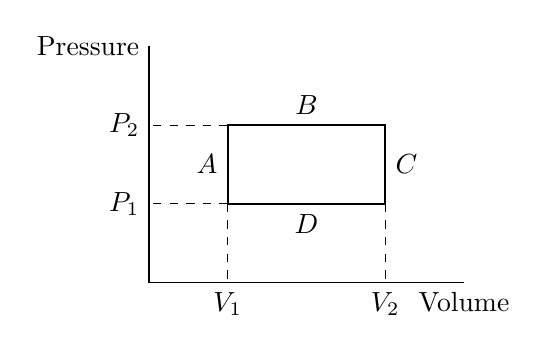
\begin{tikzpicture}
			\draw(0, 0) -- (4, 0) node[below] {Volume}; 
			\draw(0, 0) -- (0, 3) node[left] {Pressure};
			\draw[thick] (1, 1) -- node[midway, left] {$A$} (1, 2) -- node[midway,above] {$B$} (3, 2) --
				node[midway, right] {$C$} (3, 1) -- node[midway,below] {$D$} cycle;
			\draw[dashed] (1, 1) -- (1, 0) node[below] {$V_1$};
			\draw[dashed] (3, 1) -- (3, 0) node[below] {$V_2$};
			\draw[dashed] (1, 1) -- (0, 1) node[left] {$P_1$};
			\draw[dashed] (1, 2) -- (0, 2) node[left] {$P_2$};
		\end{tikzpicture}
	\end{center}

	\begin{enumerate}[label=\alph*)]
		\item For each of the four steps $A$ through $D$, compute the work done on the gas, the heat added to the
			gas, and the change in energy content of the gas. Express all answers in terms of $P_1, P_2, V_1$ 
			and $V_2$. (Hint: Compute $\Delta U$ before $Q$, using the ideal gas law and the equipartition
			theorem.)

			\begin{solution}
				Let's start with process $A$. It occurs at constant volume, so therefore there is no work 
				done on or to the gas. Therefore, all the energy added into the gas (since it's 
				increasing in pressure) is going toward the internal energy. Therefore:
				\[
				\Delta U = \Delta\left( \frac{f}{2}NkT \right) = Q
				\] 
				Then, we can replace $T$ using the ideal gas law: $T = \frac{PV}{Nk}$, and also use the 
				fact that $f = 5$ since we're dealing with a diatomic gas to get:
				\[
				Q = \frac{5}{2}Nk\left( \frac{P_2V_1}{Nk} - \frac{P_1V_1}{Nk}\right) = \frac{5}{2}V_1(P_2 - P_1) = \Delta U
				\] 
				Moving on to process $B$. It occurs at constant pressure, meaning that work is being done by the 
				gas to expand from $V_1$ to $V_2$, which is $W = -P_2(V_2 - V_1)$.\footnote{I denote work as 
				negative when work is being done \textit{by} the gas.}
				Again writing out the change in internal energy:
				\[
				\Delta U = Q + W = Q - P_2(V_2 - V_1)
				\] 
				Then using the equipartition theorem $\Delta U = \Delta\left( \frac{f}{2}NkT \right)$, 
				we have:
				\[
				Q = \frac{f}{2}Nk\frac{P_2(V_2 - V_1)}{Nk} + P_2(V_2 - V_1) = \frac{7}{2}P_2(V_2 - V_1)
				\] 
				This also means that the change in internal energy can be written as:
				\[
				\Delta U = \frac{7}{2}P_2(V_2 - V_1) - P_2(V_2 - V_1) = \frac{5}{2}(V_2 - V_1)
				\] 
				For process $C$, this is the same process as $A$ except in reverse, so we can 
				basically just copy over the formula while switching the initial and final values:
				\[
				\Delta U = Q = \frac{5}{2}V_2(P_1 - P_2)
				\] 
				(Note that the sign is encoded in $P_1 - P_2$.) Further, we know for the same reasons in $A$ that
				there is no work done by or to the gas since 
				it's being held at constant volume, so all this heat contributes to decreasing the internal
				energy. For process $D$, this is the same as process $B$ but in reverse, so here work is 
				being done to the gas, hence $W = -P_1(V_1 - V_2)$. Now using equipartition theorem with 
				the ideal gas law:
				\[
					\Delta U = Q + W = Q - P_1(V_1 - V_2) 				
				\] 
				Therefore, we can write
				\[
					Q = \frac{f}{2}Nk\frac{P_1(V_1 - V_2)}{Nk}  + P_1(V_1 - V_2) = \frac{7}{2}P_1(V_1 - V_2)
				\]		
				Note that here, $Q$ is negative since the heat is escaping the system. Also, just like 
				process $B$, the change in internal energy can be written as:
				\[
				\Delta U = \frac{7}{2}P_1(V_1 - V_2) - P_1( V_1 - V_2) = \frac{5}{2}P_1(V_1 - V_2) 
				\] 
			\end{solution}
		\item Describe in words what is physically being done during each of the four steps; for example, 
			during step $A$, heat is added to the gas (from an external flame or something) while 
			the piston is held fixed.

			\begin{solution}
				As described in the problem, we know that in process $A$ heat is added to the gas while the
				piston is held fixed. Now for the other three processes:
				\begin{itemize}
					\item Process B: Heat is added into the system, and the piston is let go to allow for 
						the gas to expand. 
					\item Process C: Heat is removed (using an ice bath for instance), while the piston is held 
						fixed.
					\item Process D: Heat is removed, and the piston is allowed to move.
				\end{itemize}
			\end{solution}
		\item Compute the net work done on the gas, the net heat added to the gas, and the net change 
			in energy of the gas during the entire cycle. Are the results as you expected? Explain 
			briefly. 

			\begin{solution}
				To calculate the net work on the gas, we note first that processes B and D are the only 
				processes that contain nonzero work, since the other two are done at constant volume. Computing
				the works:
				\begin{align*}
					W_B &= -P\Delta V = -P_2(V_2 - V_1)\\
					W_D &= -P\Delta V = -P_1(V_1 - V_2) 
				\end{align*}
				So to find the net work done, let's add these two up:
				\[
					W_{\text{net}} = W_B + W_D = -P_2(V_2 - V_1) + P_1(V_2 - V_1) = (V_2 - V_1)(P_1 - P_2)
				\] 
				Since $P_2 > P_1$ according to the diagram, we conclude that $W_{\text{net}} < 0$, so 
				there is more work done on the surroundings by the gas than the surroundings to the gas.

				Now we need to compute the net heat added to the gas. To do this, we just add up the heats:
				\begin{align*}
					Q_{\text{net}} &= \frac{5}{2}V_1(P_2 - P_1) + \frac{3}{2}P_2(V_2 - V_1) + 
					\frac{5}{2}V_2(P_1 - P_2) + \frac{3}{2}P_1(V_1 - V_2)\\
					&= \frac{5}{2}(V_1 - V_2)(P_2 - P_1) + \frac{3}{2}(V_2 - V_1)(P_2 - P_1) \\
					&= \left( \frac{5}{2} - \frac{3}{2} \right) (V_1 - V_2)(P_2 - P_1) \\
					&= (V_1 - V_2)(P_2 - P_1) 
				\end{align*} 
				Since $V_2 > V_1$, we get that the net heat added is negative, and exactly equal in magnitude
				to the amount of work done by the gas. This tracks perfectly with the conservation of energy. 
				As for the net energy change, we note that $\Delta U > 0$ in processes $A$ and $B$, whereas 
				they are negative in $C$ and $D$. Computing these exactly:
				\[
					\Delta U_{\text{net}} = \frac{5}{2}V_1(P_2 - P_1) + \frac{5}{2}P_2(V_2 - V_1) + \frac{5}{2}
					V_2(P_1 - P_2) + \frac{5}{2}P_1(V_1 - V_2)
				\] 
				Rewriting this slightly:
				\begin{align*}
					\Delta U_{\text{net}} &= \frac{5}{2}V_1(P_2 - P_1) - \frac{5}{2}V_2(P_2 - P_1) + 
					\frac{5}{2}P_2(V_2 - V_1) - \frac{5}{2}P_1(V_2 - V_1)\\
					&= -\frac{5}{2}(P_2 - P_1)(V_2 - V_1) + \frac{5}{2}(V_2 - V_1)(P_2 - P_1) \\
					&= 0 
				\end{align*} 
				This also makes sense, since the diagram ends exactly where it started, therefore the state 
				of the gas should be the same as when the cycle started. This implies that the initial and final
				states should have the same internal energy, exactly as suggested by $\Delta U = 0$.
			\end{solution}
	\end{enumerate}
	\pagebreak
	\section*{Schroeder 1.38 (5 pts)}
	Two identical bubbles of gas form at the bottom of a lake, then rise to the surface. Because the pressure
	is much lower at the surface than at the bottom, both bubbles expand as they rise. However, bubble $A$ 
	rises very quickly, so that no heat is exchanged between it and the water. Meanwhile, bubble $B$ rises 
	slowly (impeded by a tangle of seaweed), so that it always remains in thermal equilibrium with the water 
	(which has the same temperature everywhere). Which of the two bubbles is larger by the time they reach the 
	surface? Explain your reasoning fully.

	\begin{solution}
		Let's look at bubble $B$ first. As $B$ expands, since it expands isothermally, heat is constantly 
		being exchanged between the air inside the bubble and the surrounding water. As the bubble expands, 
		it is also doing work on the surrounding water, but this work is also being compensated by the heat 
		flowing into the bubble from the water:
		\[
		\Delta U_B = Q + W
		\] 
		So even though here $W$ takes away internal energy from the bubble, the $Q$ is positive just enough so 
		that $\Delta U = 0$.

		Compare this to bubble $A$, which rises adiabatically. It still does work on the environment since 
		it expands, and since they reach the same final pressure they both expand by the same amount. However, 
		since there is no heat transfer (by definition of an adiabatic process), then the change in internal 
		energy of bubble $A$ cannot be offset by heat exchange. Thus, for bubble $A$:
		\[
		\Delta U_A = W < 0
		\] 
		Since the size of the bubble is directly influenced by its internal energy (due to $PV = NkT$ and 
		$U = \frac{f}{2}NkT$), then the bubble with higher energy will also be the larger of the two. Therefore, 
		since the change in energy of bubble $B$ is zero whereas bubble $A$ is negative, then we conclude 
		that bubble $B$ must be larger.
	\end{solution}

%	\pagebreak

%	\section*{Scheoder 1.39 (15 pts)}
%	By applying Newton's laws to the oscillations of a continuous medium, one can show that the speed of a sound 
%	wave is given by 
%	\[
%	c_s = \sqrt{\frac{B}{\rho}} 
%	\] 
%	where $\rho$ is the density of the medium (mass per unit volume) and $B$ is the \textbf{bulk modulus}, a 
%	measure of the medium's stiffness. MOre precisely, if we imagine applying an increase in pressure $\Delta P$ 
%	to a chunk of the material, and this increase results in a (negative) change in volume $\Delta V$, 
%	then $B$ is defined as the change in pressure divided by the magnitude of the fractional change in volume:
%	\[
%	B \equiv \frac{\Delta P}{-\Delta V / V}
%	\] 
%	This definition is \textit{still} ambiguous, however, because I haven't said whether the compression is to
%	take place isothermally or adiabatically (or in some other way).
%	\begin{enumerate}[label=\alph*)]
%		\item Compute the bulk modulus of an ideal gas, in terms of its pressure $P$, for 
%			both isothermal and adiabatic compression.
%		\item Argue that for purposes of computing the speed of a sound wave, the \textit{adiabatic} $B$ 
%			is the one we should use.
%		\item Derive an expression for the speed of sound in an ideal gas, in terms of its temperature and 
%			average molecular mass. Compare your result to the formula for the rms speed of the omolecules in 
%			the gas. Evaluate the speed of sound numerically at room temperature.
%		\item When Scotland's Battlefield Band played in Utah, one musician remarked that the high altitude
%			threw their bagpipes out of tune. Would you expect the altitude ot affect the speed of sound (and 
%			hence the frequencies of the standing waves in pipes)? If so, in which direction? If not, why not? 
%	\end{enumerate}
\end{document}

